\Opensolutionfile{solutions}[ex]
\section*{Exercises}

\begin{enumialphparenastyle}

\begin{ex}  Find the matrix for the linear transformation which
rotates every vector in $\mathbb{R}^{2}$ through an angle of $\pi /3.$
\begin{sol}
$\leftB
\begin{array}{cc}
\cos \left(
\frac{\pi }{3}\right) & -\sin \left( \frac{\pi }{3}\right) \\
\sin \left( \frac{\pi }{3}\right) & \cos \left( \frac{\pi }{3}\right)%
\end{array}
\rightB = \leftB
\begin{array}{cc}
\frac{1}{2} & -\frac{1}{2}\sqrt{3} \\
\frac{1}{2}\sqrt{3} & \frac{1}{2}
\end{array}
\rightB $
\end{sol}
\end{ex}


\begin{ex} Find the matrix for the linear transformation which rotates every
vector in $\mathbb{R}^{2}$ through an angle of $\pi /4.$
\begin{sol}
$\leftB
\begin{array}{cc}
\cos \left( \frac{\pi }{4}\right) & -\sin \left( \frac{\pi }{4}\right) \\
\sin \left( \frac{\pi }{4}\right) & \cos \left( \frac{\pi }{4}\right)
\end{array}
\rightB = \leftB
\begin{array}{cc}
\frac{1}{2}\sqrt{2} & -\frac{1}{2}\sqrt{2} \\
\frac{1}{2}\sqrt{2} & \frac{1}{2}\sqrt{2}
\end{array}
\rightB $
\end{sol}
\end{ex}

\begin{ex} Find the matrix for the linear transformation which rotates every
vector in $\mathbb{R}^{2}$ through an angle of $-\pi /3.$
\begin{sol}
$\leftB
\begin{array}{cc}
\cos \left( -\frac{\pi }{3}\right) & -\sin \left( -\frac{\pi }{3}\right) \\
\sin \left( -\frac{\pi }{3}\right) & \cos \left( -\frac{\pi }{3}\right)
\end{array}
\rightB = \leftB
\begin{array}{cc}
\frac{1}{2} & \frac{1}{2}\sqrt{3} \\
-\frac{1}{2}\sqrt{3} & \frac{1}{2}
\end{array}
\rightB $
\end{sol}
\end{ex}

\begin{ex} Find the matrix for the linear transformation which rotates every
vector in $\mathbb{R}^{2}$ through an angle of $2\pi /3.$
\begin{sol}
$\leftB
\begin{array}{cc}
\cos \left( \frac{2\pi }{3}\right) & -\sin \left( \frac{2\pi }{3}\right) \\
\sin \left( \frac{2\pi }{3}\right) & \cos \left( \frac{2\pi }{3}\right)
\end{array}
\rightB = \leftB
\begin{array}{cc}
-\frac{1}{2} & -\frac{1}{2}\sqrt{3} \\
\frac{1}{2}\sqrt{3} & -\frac{1}{2}
\end{array}
\rightB $
\end{sol}
\end{ex}

\begin{ex} Find the matrix for the linear transformation which rotates every
vector in $\mathbb{R}^{2}$ through an angle of $\pi /12.$ \textbf{Hint:\ }
Note that $\pi /12=\pi /3-\pi /4.$
\begin{sol}
\begin{eqnarray*}
&&\leftB
\begin{array}{cc}
\cos \left( \frac{\pi }{3}\right)  & -\sin \left( \frac{\pi }{3}\right)  \\
\sin \left( \frac{\pi }{3}\right)  & \cos \left( \frac{\pi }{3}\right)
\end{array}
\rightB \leftB
\begin{array}{cc}
\cos \left( -\frac{\pi }{4}\right)  & -\sin \left( -\frac{\pi }{4}\right)
\\
\sin \left( -\frac{\pi }{4}\right)  & \cos \left( -\frac{\pi }{4}\right)
\end{array}
\rightB  \\
&=&\leftB
\begin{array}{cc}
\frac{1}{4}\sqrt{2}\sqrt{3}+\frac{1}{4}\sqrt{2} & \frac{1}{4}\sqrt{2}-\frac{1
}{4}\sqrt{2}\sqrt{3} \\
\frac{1}{4}\sqrt{2}\sqrt{3}-\frac{1}{4}\sqrt{2} & \frac{1}{4}\sqrt{2}\sqrt{3}
+\frac{1}{4}\sqrt{2}
\end{array}
\rightB
\end{eqnarray*}
\end{sol}
\end{ex}

\begin{ex} Find the matrix for the linear transformation which rotates every
vector in $\mathbb{R}^{2}$ through an angle of $2\pi /3$ and then reflects
across the $x$ axis.
\begin{sol}
\[
\leftB
\begin{array}{rr}
1 & 0 \\
0 & -1
\end{array}
\rightB \leftB
\begin{array}{cc}
\cos \left( \frac{2\pi }{3}\right)  & -\sin \left( \frac{2\pi }{3}\right)
\\
\sin \left( \frac{2\pi }{3}\right)  & \cos \left( \frac{2\pi }{3}\right)
\end{array}
\rightB = \leftB
\begin{array}{cc}
-\frac{1}{2} & -\frac{1}{2}\sqrt{3} \\
-\frac{1}{2}\sqrt{3} & \frac{1}{2}
\end{array}
\rightB
\]
\end{sol}
\end{ex}

\begin{ex} Find the matrix for the linear transformation which rotates every
vector in $\mathbb{R}^{2}$ through an angle of $\pi /3$ and then reflects
across the $x$ axis.
\begin{sol}
\[
\leftB
\begin{array}{rr}
1 & 0 \\
0 & -1
\end{array}
\rightB \leftB
\begin{array}{cc}
\cos \left( \frac{\pi }{3}\right)  & -\sin \left( \frac{\pi }{3}\right)  \\
\sin \left( \frac{\pi }{3}\right)  & \cos \left( \frac{\pi }{3}\right)
\end{array}
\rightB = \leftB
\begin{array}{cc}
\frac{1}{2} & -\frac{1}{2}\sqrt{3} \\
-\frac{1}{2}\sqrt{3} & -\frac{1}{2}
\end{array}
\rightB
\]
\end{sol}
\end{ex}

\begin{ex} Find the matrix for the linear transformation which rotates every
vector in $\mathbb{R}^{2}$ through an angle of $\pi /4$ and then reflects
across the $x$ axis.
\begin{sol}
\[
\leftB
\begin{array}{rr}
1 & 0 \\
0 & -1
\end{array}
\rightB \leftB
\begin{array}{cc}
\cos \left( \frac{\pi }{4}\right)  & -\sin \left( \frac{\pi }{4}\right)  \\
\sin \left( \frac{\pi }{4}\right)  & \cos \left( \frac{\pi }{4}\right)
\end{array}
\rightB  =  \leftB
\begin{array}{cc}
\frac{1}{2}\sqrt{2} & -\frac{1}{2}\sqrt{2} \\
-\frac{1}{2}\sqrt{2} & -\frac{1}{2}\sqrt{2}
\end{array}
\rightB
\]
\end{sol}
\end{ex}

\begin{ex} Find the matrix for the linear transformation which rotates every
vector in $\mathbb{R}^{2}$ through an angle of $\pi /6$ and then reflects
across the $x$ axis followed by a reflection across the $y$ axis.
\begin{sol}
\[
\leftB
\begin{array}{rr}
-1 & 0 \\
0 & 1
\end{array}
\rightB \leftB
\begin{array}{cc}
\cos \left( \frac{\pi }{6}\right)  & -\sin \left( \frac{\pi }{6}\right)  \\
\sin \left( \frac{\pi }{6}\right)  & \cos \left( \frac{\pi }{6}\right)
\end{array}
\rightB = \leftB
\begin{array}{cc}
-\frac{1}{2}\sqrt{3} & \frac{1}{2} \\
\frac{1}{2} & \frac{1}{2}\sqrt{3}
\end{array}
\rightB
\]
\end{sol}
\end{ex}

\begin{ex} Find the matrix for the linear transformation which reflects every
vector in $\mathbb{R}^{2}$ across the $x$ axis and then rotates every vector
through an angle of $\pi /4$.
\begin{sol}
\[
\leftB
\begin{array}{cc}
\cos \left( \frac{\pi }{4}\right)  & -\sin \left( \frac{\pi }{4}\right)  \\
\sin \left( \frac{\pi }{4}\right)  & \cos \left( \frac{\pi }{4}\right)
\end{array}
\rightB \leftB
\begin{array}{rr}
1 & 0 \\
0 & -1
\end{array}
\rightB = \leftB
\begin{array}{cc}
\frac{1}{2}\sqrt{2} & \frac{1}{2}\sqrt{2} \\
\frac{1}{2}\sqrt{2} & -\frac{1}{2}\sqrt{2}
\end{array}
\rightB
\]
\end{sol}
\end{ex}

\begin{ex} Find the matrix for the linear transformation which reflects every
vector in $\mathbb{R}^{2}$ across the $y$ axis and then rotates every vector
through an angle of $\pi /4$.
\begin{sol}
\[
\leftB
\begin{array}{cc}
\cos \left( \frac{\pi }{4}\right)  & -\sin \left( \frac{\pi }{4}\right)  \\
\sin \left( \frac{\pi }{4}\right)  & \cos \left( \frac{\pi }{4}\right)
\end{array}
\rightB \leftB
\begin{array}{rr}
-1 & 0 \\
0 & 1
\end{array}
\rightB = \leftB
\begin{array}{cc}
-\frac{1}{2}\sqrt{2} & -\frac{1}{2}\sqrt{2} \\
-\frac{1}{2}\sqrt{2} & \frac{1}{2}\sqrt{2}
\end{array}
\rightB
\]
\end{sol}
\end{ex}

\begin{ex} Find the matrix for the linear transformation which reflects every
vector in $\mathbb{R}^{2}$ across the $x$ axis and then rotates every vector
through an angle of $\pi /6$.
\begin{sol}
\[
\leftB
\begin{array}{cc}
\cos \left( \frac{\pi }{6}\right)  & -\sin \left( \frac{\pi }{6}\right)  \\
\sin \left( \frac{\pi }{6}\right)  & \cos \left( \frac{\pi }{6}\right)
\end{array}
\rightB \leftB
\begin{array}{rr}
1 & 0 \\
0 & -1
\end{array}
\rightB =  \leftB
\begin{array}{cc}
\frac{1}{2}\sqrt{3} & \frac{1}{2} \\
\frac{1}{2} & -\frac{1}{2}\sqrt{3}
\end{array}
\rightB
\]
\end{sol}
\end{ex}

\begin{ex} Find the matrix for the linear transformation which reflects every
vector in $\mathbb{R}^{2}$ across the $y$ axis and then rotates every vector
through an angle of $\pi /6$.
\begin{sol}
\[
\leftB
\begin{array}{cc}
\cos \left( \frac{\pi }{6}\right)  & -\sin \left( \frac{\pi }{6}\right)  \\
\sin \left( \frac{\pi }{6}\right)  & \cos \left( \frac{\pi }{6}\right)
\end{array}
\rightB \leftB
\begin{array}{rr}
-1 & 0 \\
0 & 1
\end{array}
\rightB = \leftB
\begin{array}{cc}
-\frac{1}{2}\sqrt{3} & -\frac{1}{2} \\
-\frac{1}{2} & \frac{1}{2}\sqrt{3}
\end{array}
\rightB
\]
\end{sol}
\end{ex}

\begin{ex} Find the matrix for the linear transformation which rotates every
vector in $\mathbb{R}^{2}$ through an angle of $5\pi /12.$ \textbf{Hint:\ }
Note that $5\pi /12=2\pi /3-\pi /4.$
\begin{sol}
\[
\leftB
\begin{array}{cc}
\cos \left( \frac{2\pi }{3}\right) & -\sin \left( \frac{2\pi }{3}\right) \\
\sin \left( \frac{2\pi }{3}\right) & \cos \left( \frac{2\pi }{3}\right)
\end{array}
\rightB \leftB
\begin{array}{cc}
\cos \left( -\frac{\pi }{4}\right) & -\sin \left( -\frac{\pi }{4}\right) \\
\sin \left( -\frac{\pi }{4}\right) & \cos \left( -\frac{\pi }{4}\right)
\end{array}
\rightB = 
\]
\[
\leftB
\begin{array}{cc}
\frac{1}{4}\sqrt{2}\sqrt{3}-\frac{1}{4}\sqrt{2} & -\frac{1}{4}\sqrt{2}\sqrt{3
}-\frac{1}{4}\sqrt{2} \\
\frac{1}{4}\sqrt{2}\sqrt{3}+\frac{1}{4}\sqrt{2} & \frac{1}{4}\sqrt{2}\sqrt{3}
-\frac{1}{4}\sqrt{2}
\end{array}
\rightB
\]
Note that it doesn't matter about the order in this case.
\end{sol}
\end{ex}

\begin{ex} Find the matrix of the linear transformation which rotates every
vector in $\mathbb{R}^{3}$ counter clockwise about the $z$ axis when viewed
from the positive $z$ axis through an angle of 30$^{\circ }$ and then
reflects through the $xy$ plane.
\begin{sol}
\[
\leftB
\begin{array}{rrr}
1 & 0 & 0 \\
0 & 1 & 0 \\
0 & 0 & -1
\end{array}
\rightB \leftB
\begin{array}{ccc}
\cos \left( \frac{\pi }{6}\right)  & -\sin \left( \frac{\pi }{6}\right)  & 0
\\
\sin \left( \frac{\pi }{6}\right)  & \cos \left( \frac{\pi }{6}\right)  & 0
\\
0 & 0 & 1
\end{array}
\rightB = \leftB
\begin{array}{ccc}
\frac{1}{2}\sqrt{3} & -\frac{1}{2} & 0 \\
\frac{1}{2} & \frac{1}{2}\sqrt{3} & 0 \\
0 & 0 & -1
\end{array}
\rightB
\]
\end{sol}
\end{ex}
 
\begin{ex} Let $\vect{u}=\leftB 
\begin{array}{r}
a \\
b
\end{array}
\rightB $ be a unit vector in $\mathbb{R}^{2}.$ Find the matrix
\index{reflection!across a given vector} which reflects all vectors across
this vector, as shown in the following picture. 

\begin{center}
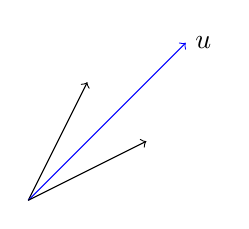
\begin{tikzpicture}
\draw[->](0,0)--(0.75,1.5);
\draw[blue, ->](0,0)--(2,2);
\draw[->](0,0)--(1.5,0.75);
\node[right] at (2,2){$\vect{u}$};
\end{tikzpicture}
\end{center}


\textbf{Hint:\ }Notice that $\leftB 
\begin{array}{r}
a \\
b
\end{array}
\rightB =\leftB
\begin{array}{c}
\cos \theta  \\
\sin \theta 
\end{array}
\rightB $ for some $\theta .$ First rotate through $-\theta .$ Next reflect through the $x$ axis. Finally rotate
through $\theta $. 
\begin{sol}
\begin{eqnarray*}
&&\leftB
\begin{array}{cc}
\cos \left( \theta \right) & -\sin \left( \theta \right) \\
\sin \left( \theta \right) & \cos \left( \theta \right)
\end{array}
\rightB \leftB
\begin{array}{rr}
1 & 0 \\
0 & -1
\end{array}
\rightB \leftB
\begin{array}{cc}
\cos \left( -\theta \right) & -\sin \left( -\theta \right) \\
\sin \left( -\theta \right) & \cos \left( -\theta \right)
\end{array}
\rightB \\
&=& \leftB
\begin{array}{cc}
\cos ^{2}\theta -\sin ^{2}\theta & 2\cos \theta \sin \theta \\
2\cos \theta \sin \theta & \sin ^{2}\theta -\cos ^{2}\theta%
\end{array}
\rightB
\end{eqnarray*}
Now to write in terms of $\left( a,b\right) ,$ note that $a/\sqrt{a^{2}+b^{2}
}=\cos \theta ,b/\sqrt{a^{2}+b^{2}}=\sin \theta .$ Now plug this in to the
above. The result is
\[
\leftB
\begin{array}{cc}
\frac{a^{2}-b^{2}}{a^{2}+b^{2}} & 2\frac{ab}{a^{2}+b^{2}} \\
2\frac{ab}{a^{2}+b^{2}} & \frac{b^{2}-a^{2}}{a^{2}+b^{2}}
\end{array}
\rightB =\frac{1}{a^{2}+b^{2}}\leftB
\begin{array}{cc}
a^{2}-b^{2} & 2ab \\
2ab & b^{2}-a^{2}
\end{array}
\rightB
\]
Since this is a unit vector, $a^{2}+b^{2}=1$ and so you get
\[
\leftB
\begin{array}{cc}
a^{2}-b^{2} & 2ab \\
2ab & b^{2}-a^{2}
\end{array}
\rightB
\]
\end{sol}
\end{ex}

\end{enumialphparenastyle}